\section{EUTXO}

\begin{frame}{UTXO vs EUTXO}
  \centering
  \begin{tikzpicture}
    \utxo
  \end{tikzpicture}
  \vspace{.5cm}
  \hfil\rule{.9\textwidth}{.4pt}\hfil
  \begin{tikzpicture}
    \eutxo
  \end{tikzpicture}
\end{frame}

% maybe add slides for data-values and contract-continuity

\begin{frame}{Running Example: Asynchronous Multi-signature Contract}
  \centering
  \begin{tikzpicture}
    \multisig
  \end{tikzpicture}

  \rule{.9\textwidth}{.4pt}

  Pay value $(v)$ to payee $(p)$ until deadline $(d)$
\end{frame}

\newcommand\multisigZoom{.9}
\begin{frame}<1>[label=multisig-eutxo,plain]
  \frametitle<2>{Limitation: Initial State}
  \only<2>{\renewcommand\multisigZoom{.7}}
  \centering

  \vspace{.5cm}
  \scalebox{\multisigZoom}{
    \begin{tikzpicture}
      \multisig
    \end{tikzpicture}
  }

  \vspace{-.5cm}
  \rule{.9\textwidth}{.4pt}

  \scalebox{.8}{\vbox{
    \begin{itemize}
      \item $\delta \in \{ \msf{Holding} , \msf{Collecting} \}$
      \item $\rho \in \{ \msf{Propose} , \msf{Add} , \msf{Cancel} , \msf{Pay} \}$
    \end{itemize}
    \vspace{-.5cm}
  }}

  \rule{.9\textwidth}{.4pt}

  \scalebox{.8}{
    \begin{tikzpicture}
      \eutxo
    \end{tikzpicture}
  }
\end{frame}

\begin{frame}{Previous Work~~[The Extended UTXO Model @ WTSC'20]}
  \begin{itemize}
  \setlength\itemsep{.25cm}

  \item \textbf{Detailed description of the Extended UTXO model (EUTXO)}
  \begin{center}
  \scalebox{.7}{
    \begin{tikzpicture}
      \eutxo
    \end{tikzpicture}
  }
  \end{center}

  \item \textbf{Formalization in} \raisebox{-.5\height}{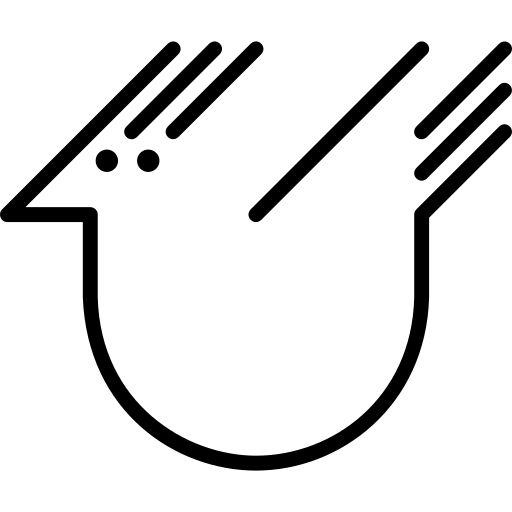
\includegraphics[height=.18\textheight]{agda}}\\

  \item \textbf{Proof of bisimulation with a Constraint Emitting Machines (CEMs)}\\
  \begin{center}
  \scalebox{.6}{
    \begin{tikzpicture}
      \multisig
    \end{tikzpicture}
  }
  \end{center}

  \end{itemize}
\end{frame}

\againframe<2>{multisig-eutxo} % talk about CEM limitation, initial states
